% Created 2023-02-10 Fri 18:06
\documentclass[9pt, b5paper]{article}
\usepackage{xeCJK}
\usepackage[T1]{fontenc}
\usepackage{bera}
\usepackage[scaled]{beraserif}
\usepackage[scaled]{berasans}
\usepackage[scaled]{beramono}
\usepackage[cache=false]{minted}
\usepackage{xltxtra}
\usepackage{graphicx}
\usepackage{xcolor}
\usepackage{multirow}
\usepackage{multicol}
\usepackage{float}
\usepackage{textcomp}
\usepackage{algorithm}
\usepackage{algorithmic}
\usepackage{latexsym}
\usepackage{natbib}
\usepackage{geometry}
\geometry{left=1.2cm,right=1.2cm,top=1.5cm,bottom=1.2cm}
\usepackage[xetex,colorlinks=true,CJKbookmarks=true,linkcolor=blue,urlcolor=blue,menucolor=blue]{hyperref}
\newminted{common-lisp}{fontsize=\footnotesize} 
\author{deepwaterooo}
\date{\today}
\title{依赖于网络异步调用的多人网络游戏}
\hypersetup{
  pdfkeywords={},
  pdfsubject={},
  pdfcreator={Emacs 28.1 (Org mode 8.2.7c)}}
\begin{document}

\maketitle
\tableofcontents


\section{因为先前的大框架还没有过关,想写一两小依赖异步网络调用的多人网络小游戏打基础.现搜集一些想法,或是现有网络项目,自己可以再加工的.}
\label{sec-1}
\begin{itemize}
\item 一个样本思路: 狠小,但大致覆盖到了几个必要的方面(通过立方体发射子弹多人游戏)
\begin{itemize}
\item \url{https://msyqgzt.gitee.io/blogs/2020/10/21/f68e6db7d782/#KCP\%E5\%8D\%8F\%E8\%AE\%AE}
\end{itemize}
\end{itemize}

\section{桢同步与状态同步}
\label{sec-2}

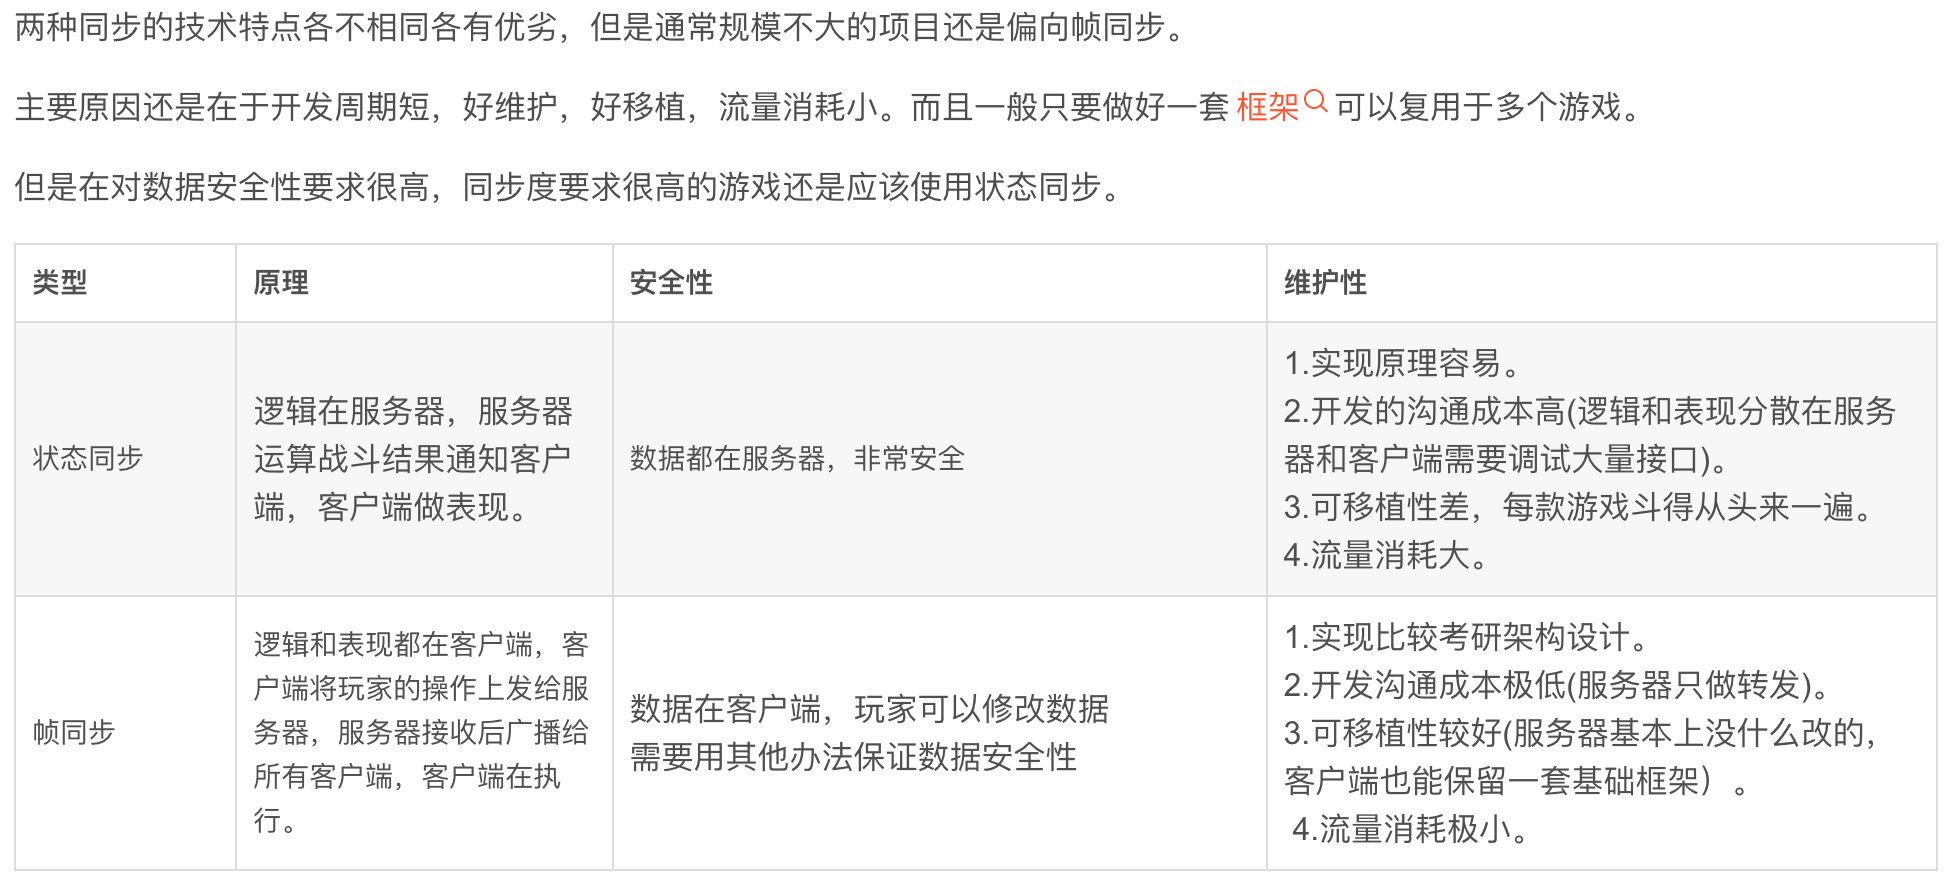
\includegraphics[width=.9\linewidth]{./pic/readme_20230209_150634.png}
\begin{itemize}
\item 当采用桢同步,当客户端的游戏规模大到一定的程度,也就是成为各种各个客户端所看到的场景不一样,因为与服务器交互所造成的各种延迟等,游戏就崩了\ldots{}..
\end{itemize}
\section{Socket 的缓冲区}
\label{sec-3}
\begin{itemize}
\item 每个 socket 被创建后,都会分配两个缓冲区,输入缓冲区和输出缓冲区。
\item write()/send() 并不立即向网络中传输数据,而是先将数据写入缓冲区中,再由TCP协议将数据从缓冲区发送到目标机器。一旦将数据写入到缓冲区,函数就可以成功返回,不管它们有没有到达目标机器,也不管它们何时被发送到网络,这些都是TCP协议负责的事情。
\item TCP协议独立于 write()/send() 函数,数据有可能刚被写入缓冲区就发送到网络,也可能在缓冲区中不断积压,多次写入的数据被一次性发送到网络,这取决于当时的网络情况、当前线程是否空闲等诸多因素,不由程序员控制。
\item read()/recv() 函数也是如此,也从输入缓冲区中读取数据,而不是直接从网络中读取,如下图所示
\end{itemize}

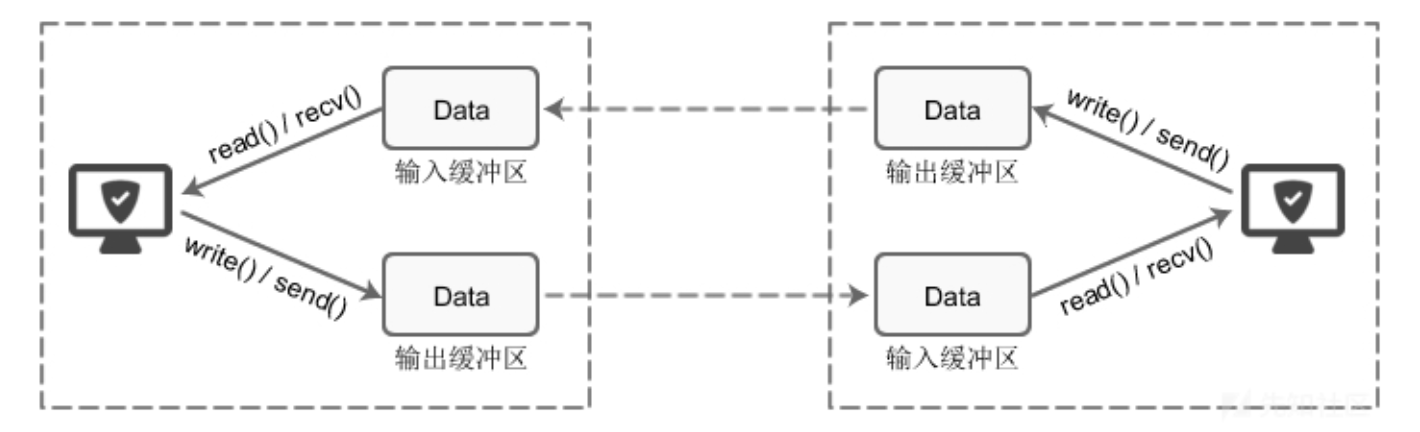
\includegraphics[width=.9\linewidth]{./pic/readme_20230210_142230.png}
\begin{itemize}
\item 这些I/O缓冲区特性如下:
\begin{itemize}
\item I/O缓冲区在每个TCP套接字中单独存在;
\item I/O缓冲区在创建套接字时自动生成;
\item 即使关闭套接字也会继续传送输出缓冲区中遗留的数据;
\item 关闭套接字将丢失输入缓冲区中的数据。
\end{itemize}
\end{itemize}

\section{几种网络调用的原理与区别}
\label{sec-4}
\subsection{KCP:}
\label{sec-4-1}

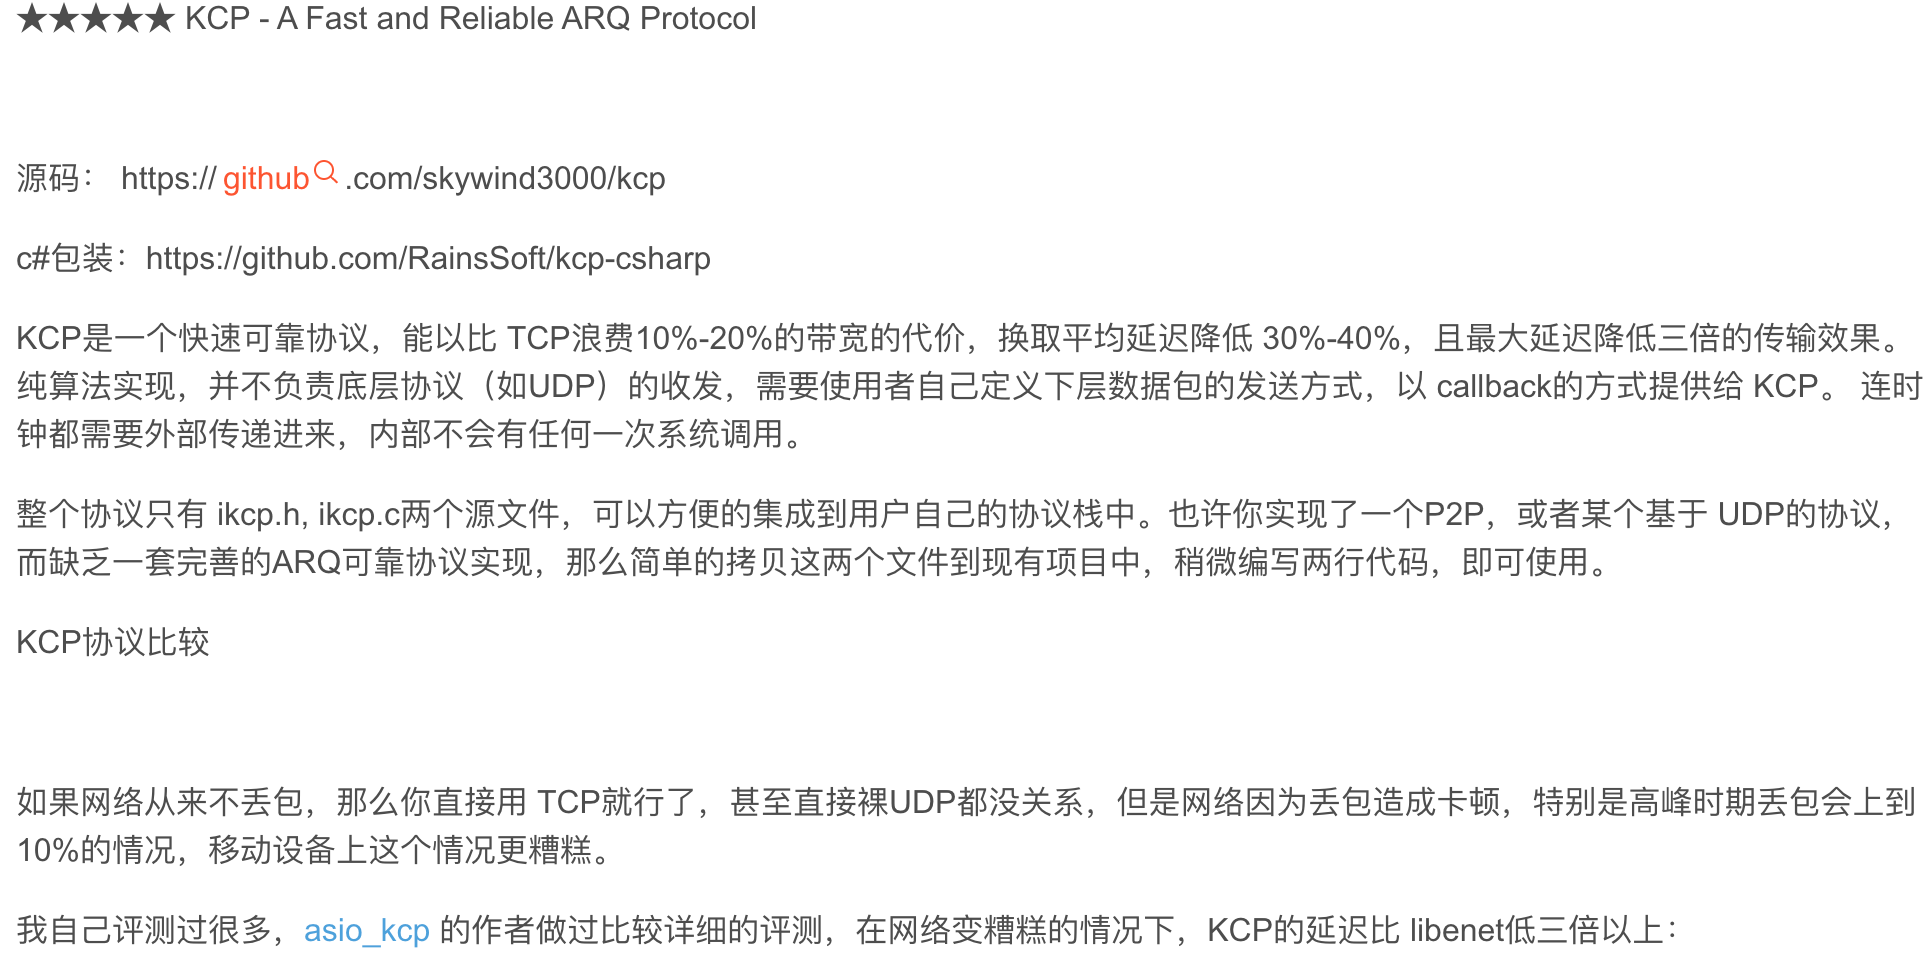
\includegraphics[width=.9\linewidth]{./pic/readme_20230210_101745.png}
\subsection{UDP :}
\label{sec-4-2}
\begin{itemize}
\item UDP的基本原理: Socket通信是典型的CS结构。服务器端为数据接受和处理方,客户端为数据请求方。首先使用C\#,我们建立服务端的启动代码。
\item 服务器端: 
\begin{minted}[fontsize=\scriptsize,linenos=false]{csharp}
// 0. 定义服务器的接收IP。这个IP应该是公开的,可以被所有访问者看到。
IPEndpoint serverIP = IPEndPoint(IPAddress.Parse("127.0.0.1"), 60010);

// 1. 定义一个Socket,协议为 UDP
Socket serverSocket = new Socket(AddressFamily.InterNetwork, SocketType.Dgram, ProtocolType.Udp);

// 2. 绑定 127.0.0.1:60010
serverSocket.Bind(IPEndPoint(IPAddress.Parse("127.0.0.1"), 60010));

// 3. 数据接收
EndPoint clientIP = new IPEndPoint(IPAddress.Any, 0);
byte[] revData = new byte[1024]; 
int len = serverSocket.ReceiveFrom(revData, ref clientIP);
string receivedData = Encoding.UTF8.GetString(revData, 0, len);
Console.WriteLine("S: Received \"{0}\" from {1}", receivedData, clientIP);

// 4. 发回数据
byte[] returnData = CurCoding.GetBytes("你好,我是服务器");
serverSocket.SendTo(returnData, sendData.Length, SocketFlags.None, clientIP);
\end{minted}
\item 说明
\begin{itemize}
\item 第0步:定义公开的IP地址和端口。地址是本机IP,而端口根据实际情况进行指定。
\item 第1步:对socket进行定义。由于要使用UDP协议,在初始化时指明 ProtocolType 为 Udp.
\item 第2步:对地址进行绑定。
\item 第3步:接收数据。这里要注意两点。
\begin{itemize}
\item 线程阻塞:调用 ReceiveFrom()以后,如果没有数据进入,线程会阻塞在这个地方,以等待数据接入。
\item 接收地址返回:通过对 ref clientIP 的引用,在收到数据后,会返回数据发送方的IP地址和端口。这里与TCP是不同的,因为在TCP协议中,是有连接的,所以IP地址是可以通过方法获得的。而UDP是无连接,所以在此获得。
\end{itemize}
\item 第4步:发回数据。根据获得的clientIP,将数据返回。
\end{itemize}
\item 客户端:
\end{itemize}
\begin{minted}[fontsize=\scriptsize,linenos=false]{csharp}
// 1. 定义一个基于UDP协议的Socket
Socket clientSocket = new Socket(AddressFamily.InterNetwork, SocketType.Dgram, ProtocolType.Udp);

// 2. 发送数据
byte[] data = Encoding.UTF8.GetBytes("你好服务器,我是客户端! ");
clientSocket.SendTo(data, data.Length, SocketFlags.None, ServerIP);

// 3. 获得返回数据。
EndPoint serverIP = new IPEndPoint(IPAddress.Any, 0);
byte[] sendData = new byte[1024];
int recv = server.ReceiveFrom(sendData, ref serverIP);
Console.WriteLine("C: Received \"{0}\" from {1}.", CurCoding.GetString(sendData, 0, recv), serverIP.ToString());

// 4. 关闭通信
clientSocket.Close();
\end{minted}
\begin{itemize}
\item 客户说明
\begin{itemize}
\item 第1步:对socket进行定义为UDP协议 。
\item 第2步:向服务器发送数据。注意:当成功发送数据后,同样也会有自己的端口可以接收数据。这点非常重要,我们可以利用这点,实现两局域网的数据通信。
\item 第3步:接收数据,同以上的服务器商。
\item 第4步:关闭socket。
\end{itemize}
\item 注意: 上面的源码极其简单,因为它采用的是同步阻塞的方式,在实际项目中用得极少,大家都用异步调用,并封装成流式写法.只给自己时时提醒一下它的原理,分不清三个的区别
\end{itemize}

\section{一个带网络请示的: 存在问题,自己也可以好好去想它存在的问题:}
\label{sec-5}
\begin{itemize}
\item \url{https://juejin.cn/post/6844903470865055758}
\item 项目存在自己的本地. 可以看下网络相关的部分.
\item \textbf{总结:} 这个项目更像是如自己现在这般开发自己的第一第二个网络多人游戏可能会存在的问题,更多的是一个设计上的天生不健全,就是多个客户端之间的同步问题,在设计之初,应该就设计为由服务器端来逻辑同步多个客户端.
\item 自己是在用unity去尝试做游戏的,中间也遇到了很多很多各种各样的问题,也都在努力去解决。到目前为止也取得了很明显的成果:主流程都是通的,现在允许多个玩家同时在线,在同一个场景中移动,转向,释放技能;服务器也能妥当的同步各个玩家的信息给所有人。不过问题也越来越多,由于现在网络通讯机制的问题,总是会出现莫名其妙的网络断开,而且断开的只是客户端接收响应的通道,客户端依然能够发给服务端消息, 服务端也可以收到,当然也正常地返回结果给客户端,然而这里客户端就收不到了。另外一个情况是:现在的同步机制是客户端各自模拟逻辑和运动,服务端只是负责同步各自的位置,某个玩家把自己的位置告知服务端,服务端再广播给所有其他玩家。这样就会有个问题,由于网络延迟的存在,不同玩家看到的场面局势是不一样的,而且现在也没有对技能释放出来的抛出物进行同步,那些火球的攻击判定也是客户端自行判断的,而且不同客户端的判断结果很有可能不一样,这已经很难再进行优化了,要改的话必须改成由服务端计算所有移动判定逻辑,客户端只负责发送指令和显示服务端推送的位置信息,自己移动时客户端不做移动,仅当传送给服务端的指令信息被处理,服务端推送给客户端位置变化的
\end{itemize}
\section{mac 上简单易用的图片修理工具(todo: 去找)}
\label{sec-6}
\section{应该自己记一个EME各个教室Spring 2023的课表,自己好比较有准备}
\label{sec-7}
\begin{itemize}
\item 下面就是字体对不齐的表现,中英文等宽字体会比较好,能够对得齐
\item 下面的二楼课表,记录可能有错,要再用一个周左右的时间再校正一下
\end{itemize}
\begin{center}
\begin{tabular}{rlllllll}
\hline
 & 星期日 & 星期一 & 星期二 & 星期三 & 星期四 & 星期五 & 星期六\\
\hline
8:30-9:30 &  &  &  &  &  & 前中后都有课 & \\
9:30-10:30 &  & 中间有课 & 有课 & 中间有 课 & 中间有课 & 不知道 & \\
10:30-11:30 &  &  &  & 有课 & 有课 & 前中后都有课 & \\
11:30-12:30 &  &  &  &  &  & 后 仍有课 & \\
\hline
1:30-2:30 &  &  &  &  & 有课 &  & \\
12:00 - 3:00 &  &  & 249有课 &  &  &  & \\
3:00 - 6:00 &  &  & 249有课 &  &  &  & \\
\hline
\end{tabular}
\end{center}
\begin{itemize}
\item macOS下,snipaste的截图质量发白,有点儿关工.用它是因为一个F1键就可以截屏,但是如果质量太差,需要解决,或是换用其它工具
\item 在自己阅读源码的过程中,无数的标记要手动转换输入法是极其麻烦的事,需要编辑器emacs 给点儿帮助,在特定加载模式,在特定键的输入后,作必要的输入法自动转换,减少人为操作误差与精力.(大家喜欢emacs, 也都是因为它的高度可订制化.)爱表哥,爱生活!!!把那个sis包弄懂,用到自己的工具中去.晚上弄
\item 下午就自己找项目,写苹果系统中的项目
\item spectacular 分屏工具的使用还是了解一下,可以提高开发效率
\item mac系统下的安卓模拟器: 没弄明白是怎么安装的?\url{https://blog.csdn.net/linxinfa/article/details/124844236}
\begin{itemize}
\item \url{https://github.com/google/android-emulator-m1-preview/releases}
\item 这个还要弄一下,因为必要的时候总是还是需要这些东西的
\end{itemize}
\end{itemize}
\section{因为对自己系统的开发环境仍然是感觉不熟悉,先试着整个小应用熟悉一下}
\label{sec-8}
\begin{itemize}
\item 想写一个麻将连连看连连打,可是无从下手,会参考别人的教程,再自己网络搜索一下,试图解决这个问题.若是实在没有图片,就用别的图片代替.
\item 麻将文: \url{https://blog.csdn.net/dlyhy/article/details/121325244?utm_medium=distribute.pc_relevant.none-task-blog-2~default~baidujs_baidulandingword~default-1-121325244-blog-120835692.pc_relevant_aa&spm=1001.2101.3001.4242.2&utm_relevant_index=4}
\item 菜单:最开始学的是Visual Basic 窗体设计与实现,但是现在全忘光了,连什么方法写在哪里都还需要再科普一下\ldots{}..但是会把它写出来
\begin{itemize}
\item \url{https://www.dongchuanmin.com/net/2540.html}
\item \url{https://www.dongchuanmin.com/net/2550.html}
\end{itemize}
\end{itemize}
% Emacs 28.1 (Org mode 8.2.7c)
\end{document}